
\chapter{Getting started}
\label{txt:gettingstarted}

Once you have your Corina desktop application installed (see chapter \ref{txt:installation}) and you also have access to a Corina server (either via your lab network administrator or your own on as a Virtual Appliance) you are ready to start using Corina.  Below are some basic instructions for performing common tasks in Corina followed by a number of more in-depth chapters.

\section{Measuring a new sample}
\index{Sample!Measuring|(}
Once your measuring platform has been configured, measuring your first sample is simple.  To start a new measurement go to \menutwo{File}{New} or click the `new' icon on the home screen. A dialog will appear where you can scan your sample's barcode, or press the button to enter metadata for your sample later. Barcodes minimize data entry errors and also speed up the process of measuring your samples. See section \ref{txt:barcodes} for more information. Once you have scanned your barcode or pressed the button, you will then be presented with an empty Corina data screen (figure \ref{fig:datascreen}).

\begin{figure}[hbtp]
  \centering
    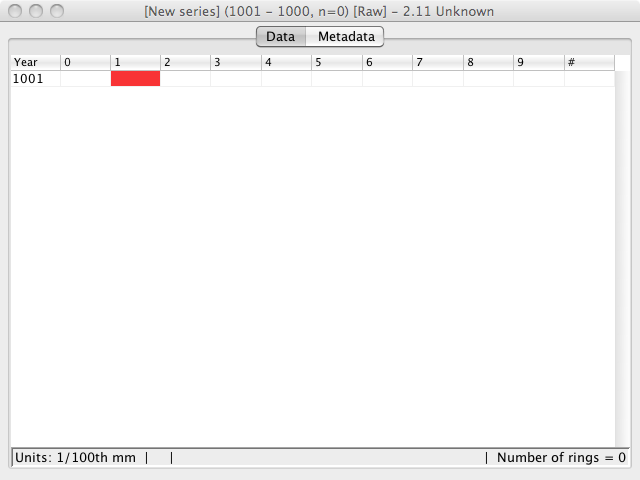
\includegraphics[width=0.6\textwidth]{Images/datascreen.png}
    \caption{An empty data window ready to receive measurements.  Note the status bar at the bottom includes buttons for changing the display units and cumulative statistics.}
    \label{fig:datascreen}
\end{figure}

The next step is to fill out the metadata tab. If you have used a barcode, nearly all of this metadata will be filled in for you, otherwise you will need to fill this out yourself. Details about metadata can be found in chapter \ref{txt:metadata}, page \pageref{txt:metadata}.

To begin measuring your sample you can now go to \menutwo{Edit}{Start measuring} or you can press F5. While measuring you should be provided with audible feedback for each ring measured with a more pronounced sound made every 10th ring. If there is a problem communicating with your measuring hardware, check your settings in the preferences dialog. If you still have problems contact the Corina developers by going to \menutwo{Help}{Report bug on last transaction}, making sure you include your email address and any further information.

Depending on the measuring platform hardware you have, you will see some variation of the measuring panel in figure \ref{fig:measurepanel}. The left display holds the absolute position of the last ring boundary (for device that measure cumulatively), the middle display holds the last recorded measurement width and the right display holds the current position of the measuring plaform (for devices that report live measurements).  The right-hand display is useful for devices that don't have a physical display such as the Lintab. 

\begin{wrapfigure}{r}{0.5\textwidth}
  \begin{center}
    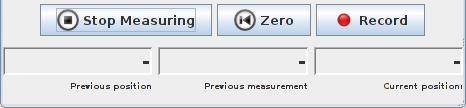
\includegraphics[width=6cm]{Images/measurepanel.png}
  \end{center}
  \caption{Measuring control panel.}
  \label{fig:measurepanel}
\end{wrapfigure}


Corina supports the measuring of rings both individually and cumulatively.  We feel that it is easier and more accurate to measure rings individually, that is to say the device is reset to zero after each measurement.  If a device accepts requests to reset measurements (e.g.\ Quadra Chek boxes) or if it automatically resets itself to zero after recording a measurement (e.g.\ EVE IO) then this procedure is used by Corina.  In this case the user begins measuring by setting the display to zero, then turns the platform to the end of the ring, then either presses the `measure' button on the hardware device or the `record' button on the screen.

\tip{If your device does not have a physical `measure' button you don't need to use the mouse in Corina to click the `record' button each time.  Use the tab key to ensure the record button is highlighted, then you can use the space bar on your keyboard instead.  This means you don't need to lift your eyes from your microscope to ensure you are clicking the button correctly.}

Certain devices (e.g. Boekler Microcode boxes) do not listen for requests to reset to zero.  In this case to measure each ring individually, you would need to manually reset the reading to zero following each measurement.  This would of course be extremely tedious.  In this situation Corina measures cumulatively from the beginning of the first ring and calculates the ring width based on the previous ring boundary position.  With this method you must be careful not to knock your sample, and you must also take special care when altering radii to navigate around problem structures.  If you do knock your sample, the best way to recover is to reset your platform to zero and press the measure button.  Next, press the `stop measuring button', manually fix the values in the data table, then begin measuring again from where you left off.


\index{Ring remarks}
While you measure your sample you can flag features in a ring by right clicking on any cell in the table and selecting one or more of the standard notes (see figure \ref{fig:ringremarks}).

Corina supports all standard TRiDaS remarks including: fire damage; frost damage; crack; false ring(s); compression wood; tension wood; traumatic ducts; single pinned; double pinned; triple pinned and many others.  Rings that include remarks are indicated by the relevant icon in the data screen.  Depending on your method of work, this can be useful for keeping track of sample pin holes.  For instance, if a missing or false ring is discovered after a sample has been pinholed, the offset in pinholes can be easily seen without resurfacing the sample.  In the future Corina will also include support for user defined ring remarks.  

\begin{wrapfigure}{r}{0.5\textwidth}
  \begin{center}
    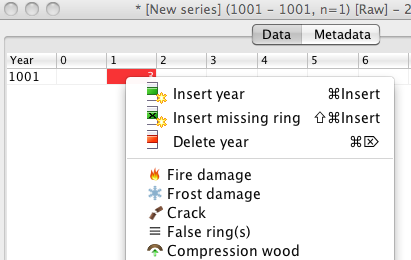
\includegraphics[width=0.42\textwidth]{Images/ringremarks.png}
  \end{center}
  \caption{Right click context menu showing some of the options for adding remarks to rings.}
  \label{fig:ringremarks}
\end{wrapfigure}

The data screen also contains a status bar at the bottom. By click on the units section, you can switch between micron and 1/100th mm units. Corina understands the units being supplied by the measuring platform, therefore changes here are purely for display purposes only. If you have a platform that measures in microns, but prefer to see the values in 1/100th mm then you can use this feature. At the bottom ring of the status bar you can choose one of a variety of summary information about your series.

Once you have finished measuring your sample, you should then go to \menutwo{File}{Save} to save your series to the database. 
\index{Sample!Measuring|)}


\section{Opening existing data}
\index{Sample!Opening}
If you have used traditional dendrochronology software, you are probably used to opening existing dendro data files from your computer.  Corina works in a different way.  All data accessed by Corina is stored within the central Corina database rather than from files.  The database provides many benefits over file based storage, most importantly it means there is a high degree of security and integrity in your data.  

To use data that you have stored in existing data files you must first \emph{import} your data into the Corina database.  This gives you the opportunity to clean-up your data!  For details of how to import your data see chapter \ref{txt:importExport}, page \pageref{txt:importExport}.

Once you have data in your database, either by importing existing data files or measuring new samples, you can access your data through the database browser.  This is accessed through the \menutwo{File}{Open} or \menutwo{File}{Open multiple} menus and an example of the dialog is shown in figure \ref{fig:dbbrowser}. The same database browser dialog is used in multiple places throughout Corina, e.g.\ when adding addition series to graphs and when choosing chronologies to crossdate against. 

\begin{figure}[hbtp]
  \centering
    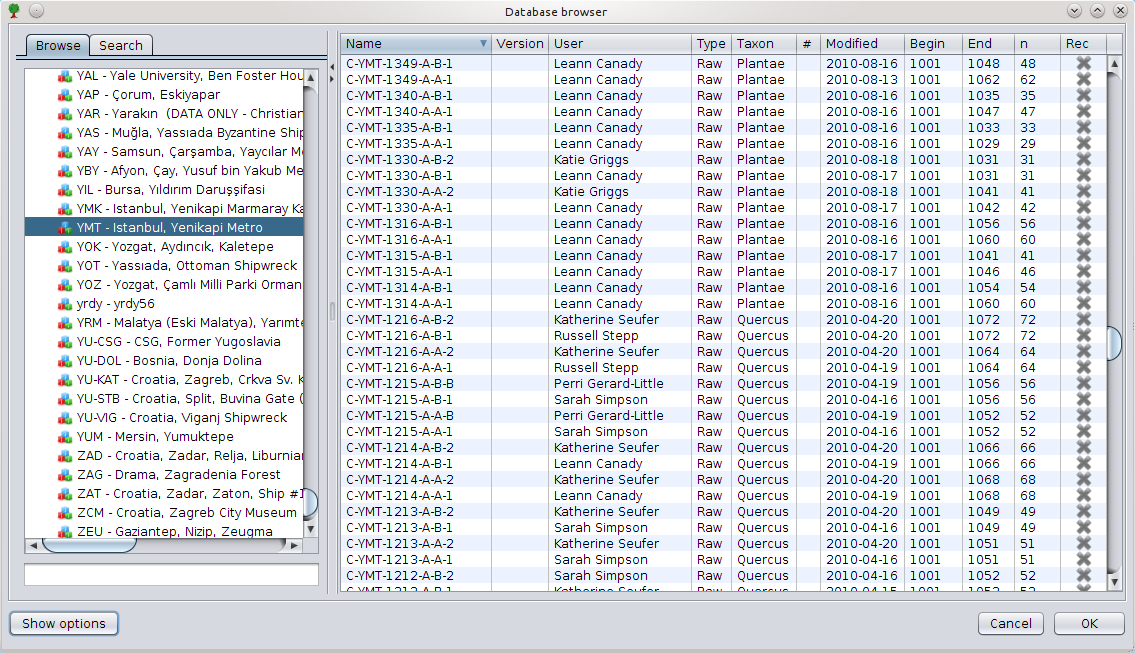
\includegraphics[width=0.9\textwidth]{Images/dbbrowser.png}
    \caption{Screenshot of the database browser dialog.}
    \label{fig:dbbrowser}
\end{figure}

The database browser is divided into two main parts.  On the left is the browse and search tabs, and on the right is the series table.  Selecting options in the browse or search tab populates the series table on the right with all the series that match the specified criteria.  

\warn{The search tab is currently a `work-in-progress' so we recommend you use the browse tab until further notice.}

The browse tab shows a heirarchical tree view of the contents of your Corina database based upon the TRiDaS data model.  The panel will be pre-populated with all the objects in your database but it is possible to `drill-down' by right clicking on an object and choosing `Expand branch'.  Expanding an object for instance, will show all the elements associated with that object, and expanding an element will show all the samples associated with the specified element.  To better understand the TRiDaS terminology please read chapter \ref{txt:metadata}, page \pageref{txt:metadata}.

By double clicking (or right clicking and choosing `Search for associated series') on an item in the browse panel Corina will search the database for all series that are associated with the specified entity.  The results of the search will be shown in the series table on the right of the screen.  This table shows basic metadata about each search and is sortable by click on any of the column headers.  To open a series, simply select one of these series and click `OK'.  If the database browser is open in 'multiple series' mode, then you can use the arrow buttons to select multiple series to open in one go.

There is also a `Show options' button on the database browser dialog.  This adds additional advanced methods for filtering the series table to help you find the data you are interested in.

\section{Reconciling data}
\index{Sample!Reconciling}
Corina has been developed not only for experience dendrochronologists, but as a tool for teaching students.  It therefore includes a comprehensive `reconciling' tool for supervisors to check the quality of measurements made by students.  The reconcile dialog does a comparison of a measurement series made by a student with a references series of the same radius measured by the supervisor.  The same dialog can also prove useful for comparing measurements from two experienced dendrochronologists when handling particularly difficult samples.

 


